\documentclass[1p]{elsarticle_modified}
%\bibliographystyle{elsarticle-num}

%\usepackage[colorlinks]{hyperref}
%\usepackage{abbrmath_seonhwa} %\Abb, \Ascr, \Acal ,\Abf, \Afrak
\usepackage{amsfonts}
\usepackage{amssymb}
\usepackage{amsmath}
\usepackage{amsthm}
\usepackage{scalefnt}
\usepackage{amsbsy}
\usepackage{kotex}
\usepackage{caption}
\usepackage{subfig}
\usepackage{color}
\usepackage{graphicx}
\usepackage{xcolor} %% white, black, red, green, blue, cyan, magenta, yellow
\usepackage{float}
\usepackage{setspace}
\usepackage{hyperref}

\usepackage{tikz}
\usetikzlibrary{arrows}

\usepackage{multirow}
\usepackage{array} % fixed length table
\usepackage{hhline}

%%%%%%%%%%%%%%%%%%%%%
\makeatletter
\renewcommand*\env@matrix[1][\arraystretch]{%
	\edef\arraystretch{#1}%
	\hskip -\arraycolsep
	\let\@ifnextchar\new@ifnextchar
	\array{*\c@MaxMatrixCols c}}
\makeatother %https://tex.stackexchange.com/questions/14071/how-can-i-increase-the-line-spacing-in-a-matrix
%%%%%%%%%%%%%%%

\usepackage[normalem]{ulem}

\newcommand{\msout}[1]{\ifmmode\text{\sout{\ensuremath{#1}}}\else\sout{#1}\fi}
%SOURCE: \msout is \stkout macro in https://tex.stackexchange.com/questions/20609/strikeout-in-math-mode

\newcommand{\cancel}[1]{
	\ifmmode
	{\color{red}\msout{#1}}
	\else
	{\color{red}\sout{#1}}
	\fi
}

\newcommand{\add}[1]{
	{\color{blue}\uwave{#1}}
}

\newcommand{\replace}[2]{
	\ifmmode
	{\color{red}\msout{#1}}{\color{blue}\uwave{#2}}
	\else
	{\color{red}\sout{#1}}{\color{blue}\uwave{#2}}
	\fi
}

\newcommand{\Sol}{\mathcal{S}} %segment
\newcommand{\D}{D} %diagram
\newcommand{\A}{\mathcal{A}} %arc


%%%%%%%%%%%%%%%%%%%%%%%%%%%%%5 test

\def\sl{\operatorname{\textup{SL}}(2,\Cbb)}
\def\psl{\operatorname{\textup{PSL}}(2,\Cbb)}
\def\quan{\mkern 1mu \triangleright \mkern 1mu}

\theoremstyle{definition}
\newtheorem{thm}{Theorem}[section]
\newtheorem{prop}[thm]{Proposition}
\newtheorem{lem}[thm]{Lemma}
\newtheorem{ques}[thm]{Question}
\newtheorem{cor}[thm]{Corollary}
\newtheorem{defn}[thm]{Definition}
\newtheorem{exam}[thm]{Example}
\newtheorem{rmk}[thm]{Remark}
\newtheorem{alg}[thm]{Algorithm}

\newcommand{\I}{\sqrt{-1}}
\begin{document}

%\begin{frontmatter}
%
%\title{Boundary parabolic representations of knots up to 8 crossings}
%
%%% Group authors per affiliation:
%\author{Yunhi Cho} 
%\address{Department of Mathematics, University of Seoul, Seoul, Korea}
%\ead{yhcho@uos.ac.kr}
%
%
%\author{Seonhwa Kim} %\fnref{s_kim}}
%\address{Center for Geometry and Physics, Institute for Basic Science, Pohang, 37673, Korea}
%\ead{ryeona17@ibs.re.kr}
%
%\author{Hyuk Kim}
%\address{Department of Mathematical Sciences, Seoul National University, Seoul 08826, Korea}
%\ead{hyukkim@snu.ac.kr}
%
%\author{Seokbeom Yoon}
%\address{Department of Mathematical Sciences, Seoul National University, Seoul, 08826,  Korea}
%\ead{sbyoon15@snu.ac.kr}
%
%\begin{abstract}
%We find all boundary parabolic representation of knots up to 8 crossings.
%
%\end{abstract}
%\begin{keyword}
%    \MSC[2010] 57M25 
%\end{keyword}
%
%\end{frontmatter}

%\linenumbers
%\tableofcontents
%
\newcommand\colored[1]{\textcolor{white}{\rule[-0.35ex]{0.8em}{1.4ex}}\kern-0.8em\color{red} #1}%
%\newcommand\colored[1]{\textcolor{white}{ #1}\kern-2.17ex	\textcolor{white}{ #1}\kern-1.81ex	\textcolor{white}{ #1}\kern-2.15ex\color{red}#1	}

{\Large $\underline{12a_{0946}~(K12a_{0946})}$}

\setlength{\tabcolsep}{10pt}
\renewcommand{\arraystretch}{1.6}
\vspace{1cm}\begin{tabular}{m{100pt}>{\centering\arraybackslash}m{274pt}}
\multirow{5}{120pt}{
	\centering
	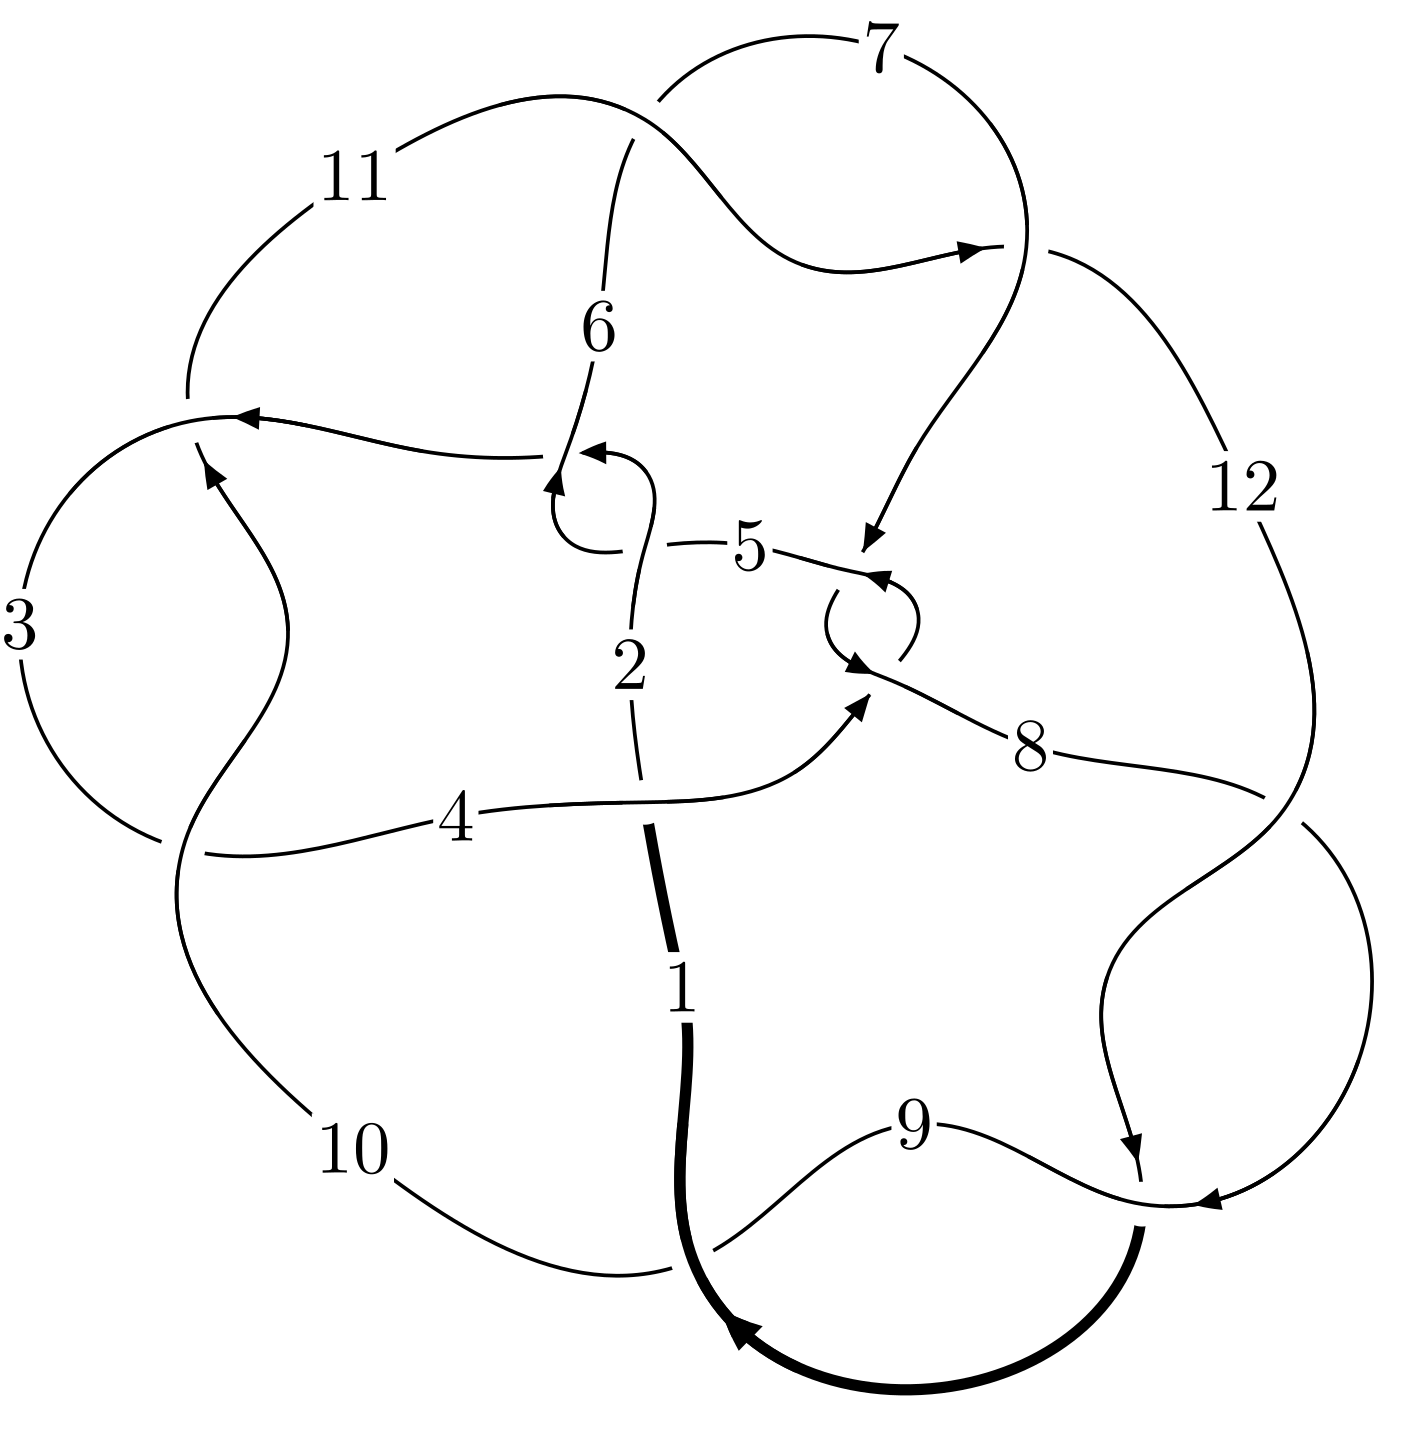
\includegraphics[width=112pt]{../../../GIT/diagram.site/Diagrams/png/1747_12a_0946.png}\\
\ \ \ A knot diagram\footnotemark}&
\allowdisplaybreaks
\textbf{Linearized knot diagam} \\
\cline{2-2}
 &
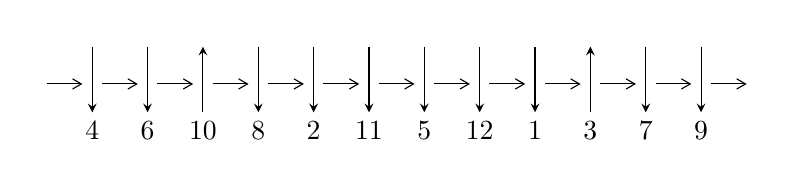
\begin{tikzpicture}[x=20pt, y=17pt]
	% nodes
	\node (C0) at (0, 0) {};
	\node (C1) at (1, 0) {};
	\node (C1U) at (1, +1) {};
	\node (C1D) at (1, -1) {4};

	\node (C2) at (2, 0) {};
	\node (C2U) at (2, +1) {};
	\node (C2D) at (2, -1) {6};

	\node (C3) at (3, 0) {};
	\node (C3U) at (3, +1) {};
	\node (C3D) at (3, -1) {10};

	\node (C4) at (4, 0) {};
	\node (C4U) at (4, +1) {};
	\node (C4D) at (4, -1) {8};

	\node (C5) at (5, 0) {};
	\node (C5U) at (5, +1) {};
	\node (C5D) at (5, -1) {2};

	\node (C6) at (6, 0) {};
	\node (C6U) at (6, +1) {};
	\node (C6D) at (6, -1) {11};

	\node (C7) at (7, 0) {};
	\node (C7U) at (7, +1) {};
	\node (C7D) at (7, -1) {5};

	\node (C8) at (8, 0) {};
	\node (C8U) at (8, +1) {};
	\node (C8D) at (8, -1) {12};

	\node (C9) at (9, 0) {};
	\node (C9U) at (9, +1) {};
	\node (C9D) at (9, -1) {1};

	\node (C10) at (10, 0) {};
	\node (C10U) at (10, +1) {};
	\node (C10D) at (10, -1) {3};

	\node (C11) at (11, 0) {};
	\node (C11U) at (11, +1) {};
	\node (C11D) at (11, -1) {7};

	\node (C12) at (12, 0) {};
	\node (C12U) at (12, +1) {};
	\node (C12D) at (12, -1) {9};
	\node (C13) at (13, 0) {};

	% arrows
	\draw[->,>={angle 60}]
	(C0) edge (C1) (C1) edge (C2) (C2) edge (C3) (C3) edge (C4) (C4) edge (C5) (C5) edge (C6) (C6) edge (C7) (C7) edge (C8) (C8) edge (C9) (C9) edge (C10) (C10) edge (C11) (C11) edge (C12) (C12) edge (C13) ;	\draw[->,>=stealth]
	(C1U) edge (C1D) (C2U) edge (C2D) (C3D) edge (C3U) (C4U) edge (C4D) (C5U) edge (C5D) (C6U) edge (C6D) (C7U) edge (C7D) (C8U) edge (C8D) (C9U) edge (C9D) (C10D) edge (C10U) (C11U) edge (C11D) (C12U) edge (C12D) ;
	\end{tikzpicture} \\
\hhline{~~} \\& 
\textbf{Solving Sequence} \\ \cline{2-2} 
 &
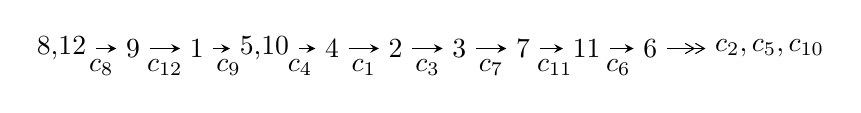
\begin{tikzpicture}[x=23pt, y=7pt]
	% node
	\node (A0) at (-1/8, 0) {8,12};
	\node (A1) at (1, 0) {9};
	\node (A2) at (2, 0) {1};
	\node (A3) at (49/16, 0) {5,10};
	\node (A4) at (33/8, 0) {4};
	\node (A5) at (41/8, 0) {2};
	\node (A6) at (49/8, 0) {3};
	\node (A7) at (57/8, 0) {7};
	\node (A8) at (65/8, 0) {11};
	\node (A9) at (73/8, 0) {6};
	\node (C1) at (1/2, -1) {$c_{8}$};
	\node (C2) at (3/2, -1) {$c_{12}$};
	\node (C3) at (5/2, -1) {$c_{9}$};
	\node (C4) at (29/8, -1) {$c_{4}$};
	\node (C5) at (37/8, -1) {$c_{1}$};
	\node (C6) at (45/8, -1) {$c_{3}$};
	\node (C7) at (53/8, -1) {$c_{7}$};
	\node (C8) at (61/8, -1) {$c_{11}$};
	\node (C9) at (69/8, -1) {$c_{6}$};
	\node (A10) at (11, 0) {$c_{2},c_{5},c_{10}$};

	% edge
	\draw[->,>=stealth]	
	(A0) edge (A1) (A1) edge (A2) (A2) edge (A3) (A3) edge (A4) (A4) edge (A5) (A5) edge (A6) (A6) edge (A7) (A7) edge (A8) (A8) edge (A9) ;
	\draw[->>,>={angle 60}]	
	(A9) edge (A10);
\end{tikzpicture} \\ 

\end{tabular} \\

\footnotetext{
The image of knot diagram is generated by the software ``\textbf{Draw programme}" developed by Andrew Bartholomew(\url{http://www.layer8.co.uk/maths/draw/index.htm\#Running-draw}), where we modified some parts for our purpose(\url{https://github.com/CATsTAILs/LinksPainter}).
}\phantom \\ \newline 
\centering \textbf{Ideals for irreducible components\footnotemark of $X_{\text{par}}$} 
 
\begin{align*}
I^u_{1}&=\langle 
1.82351\times10^{199} u^{97}-3.99104\times10^{199} u^{96}+\cdots+1.17463\times10^{197} b-5.97726\times10^{199},\\
\phantom{I^u_{1}}&\phantom{= \langle  }-8.41837\times10^{199} u^{97}+3.53183\times10^{200} u^{96}+\cdots+1.17463\times10^{197} a-7.10346\times10^{200},\\
\phantom{I^u_{1}}&\phantom{= \langle  }u^{98}-4 u^{97}+\cdots+21 u+1\rangle \\
I^u_{2}&=\langle 
-165708 u^{22}-355153 u^{21}+\cdots+96055 b-107266,\\
\phantom{I^u_{2}}&\phantom{= \langle  }89858 u^{22}+320813 u^{21}+\cdots+96055 a+622041,\;u^{23}+3 u^{22}+\cdots+5 u-1\rangle \\
\\
\end{align*}
\raggedright * 2 irreducible components of $\dim_{\mathbb{C}}=0$, with total 121 representations.\\
\footnotetext{All coefficients of polynomials are rational numbers. But the coefficients are sometimes approximated in decimal forms when there is not enough margin.}
\newpage
\renewcommand{\arraystretch}{1}
\centering \section*{I. $I^u_{1}= \langle 1.82\times10^{199} u^{97}-3.99\times10^{199} u^{96}+\cdots+1.17\times10^{197} b-5.98\times10^{199},\;-8.42\times10^{199} u^{97}+3.53\times10^{200} u^{96}+\cdots+1.17\times10^{197} a-7.10\times10^{200},\;u^{98}-4 u^{97}+\cdots+21 u+1 \rangle$}
\flushleft \textbf{(i) Arc colorings}\\
\begin{tabular}{m{7pt} m{180pt} m{7pt} m{180pt} }
\flushright $a_{8}=$&$\begin{pmatrix}1\\0\end{pmatrix}$ \\
\flushright $a_{12}=$&$\begin{pmatrix}0\\u\end{pmatrix}$ \\
\flushright $a_{9}=$&$\begin{pmatrix}1\\u^2\end{pmatrix}$ \\
\flushright $a_{1}=$&$\begin{pmatrix}- u\\- u^3+u\end{pmatrix}$ \\
\flushright $a_{5}=$&$\begin{pmatrix}716.680 u^{97}-3006.74 u^{96}+\cdots+84179.0 u+6047.37\\-155.241 u^{97}+339.769 u^{96}+\cdots+7987.50 u+508.861\end{pmatrix}$ \\
\flushright $a_{10}=$&$\begin{pmatrix}- u^2+1\\- u^4+2 u^2\end{pmatrix}$ \\
\flushright $a_{4}=$&$\begin{pmatrix}561.439 u^{97}-2666.97 u^{96}+\cdots+92166.5 u+6556.23\\-155.241 u^{97}+339.769 u^{96}+\cdots+7987.50 u+508.861\end{pmatrix}$ \\
\flushright $a_{2}=$&$\begin{pmatrix}-2232.86 u^{97}+9464.74 u^{96}+\cdots-162707. u-9052.39\\240.514 u^{97}-994.313 u^{96}+\cdots+20176.8 u+1288.64\end{pmatrix}$ \\
\flushright $a_{3}=$&$\begin{pmatrix}726.180 u^{97}-3041.76 u^{96}+\cdots+86152.2 u+6221.39\\-171.747 u^{97}+386.011 u^{96}+\cdots+8024.20 u+506.994\end{pmatrix}$ \\
\flushright $a_{7}=$&$\begin{pmatrix}-884.790 u^{97}+3739.52 u^{96}+\cdots-77156.6 u-4840.59\\574.685 u^{97}-1162.46 u^{96}+\cdots-30034.5 u-1690.30\end{pmatrix}$ \\
\flushright $a_{11}=$&$\begin{pmatrix}-2218.70 u^{97}+9267.40 u^{96}+\cdots-178246. u-10919.1\\-1006.24 u^{97}+2826.71 u^{96}+\cdots+2301.61 u-78.0343\end{pmatrix}$ \\
\flushright $a_{6}=$&$\begin{pmatrix}2277.85 u^{97}-9597.62 u^{96}+\cdots+161982. u+8982.40\\-434.686 u^{97}+1510.96 u^{96}+\cdots-17995.0 u-1202.35\end{pmatrix}$\\&\end{tabular}
\flushleft \textbf{(ii) Obstruction class $= -1$}\\~\\
\flushleft \textbf{(iii) Cusp Shapes $= -2276.86 u^{97}+4325.44 u^{96}+\cdots+123935. u+6545.69$}\\~\\
\newpage\renewcommand{\arraystretch}{1}
\flushleft \textbf{(iv) u-Polynomials at the component}\newline \\
\begin{tabular}{m{50pt}|m{274pt}}
Crossings & \hspace{64pt}u-Polynomials at each crossing \\
\hline $$\begin{aligned}c_{1}\end{aligned}$$&$\begin{aligned}
&u^{98}-15 u^{97}+\cdots+8302550 u-947299
\end{aligned}$\\
\hline $$\begin{aligned}c_{2},c_{5}\end{aligned}$$&$\begin{aligned}
&u^{98}-37 u^{96}+\cdots+5041 u-631
\end{aligned}$\\
\hline $$\begin{aligned}c_{3},c_{10}\end{aligned}$$&$\begin{aligned}
&u^{98}+u^{97}+\cdots-633 u-389
\end{aligned}$\\
\hline $$\begin{aligned}c_{4},c_{7}\end{aligned}$$&$\begin{aligned}
&u^{98}-9 u^{97}+\cdots-284 u-61
\end{aligned}$\\
\hline $$\begin{aligned}c_{6},c_{11}\end{aligned}$$&$\begin{aligned}
&u^{98}- u^{97}+\cdots+3881 u+173
\end{aligned}$\\
\hline $$\begin{aligned}c_{8},c_{9},c_{12}\end{aligned}$$&$\begin{aligned}
&u^{98}+4 u^{97}+\cdots-21 u+1
\end{aligned}$\\
\hline
\end{tabular}\\~\\
\newpage\renewcommand{\arraystretch}{1}
\flushleft \textbf{(v) Riley Polynomials at the component}\newline \\
\begin{tabular}{m{50pt}|m{274pt}}
Crossings & \hspace{64pt}Riley Polynomials at each crossing \\
\hline $$\begin{aligned}c_{1}\end{aligned}$$&$\begin{aligned}
&y^{98}-47 y^{97}+\cdots-51996320363916 y+897375395401
\end{aligned}$\\
\hline $$\begin{aligned}c_{2},c_{5}\end{aligned}$$&$\begin{aligned}
&y^{98}-74 y^{97}+\cdots-157589775 y+398161
\end{aligned}$\\
\hline $$\begin{aligned}c_{3},c_{10}\end{aligned}$$&$\begin{aligned}
&y^{98}+69 y^{97}+\cdots+1816611 y+151321
\end{aligned}$\\
\hline $$\begin{aligned}c_{4},c_{7}\end{aligned}$$&$\begin{aligned}
&y^{98}+23 y^{97}+\cdots+57570 y+3721
\end{aligned}$\\
\hline $$\begin{aligned}c_{6},c_{11}\end{aligned}$$&$\begin{aligned}
&y^{98}-91 y^{97}+\cdots-16222645 y+29929
\end{aligned}$\\
\hline $$\begin{aligned}c_{8},c_{9},c_{12}\end{aligned}$$&$\begin{aligned}
&y^{98}-102 y^{97}+\cdots-139 y+1
\end{aligned}$\\
\hline
\end{tabular}\\~\\
\newpage\flushleft \textbf{(vi) Complex Volumes and Cusp Shapes}
$$\begin{array}{c|c|c}  
\text{Solutions to }I^u_{1}& \I (\text{vol} + \sqrt{-1}CS) & \text{Cusp shape}\\
 \hline 
\begin{aligned}
u &= \phantom{-}0.869872 + 0.514495 I \\
a &= -0.048478 + 1.314500 I \\
b &= -0.088737 - 0.875286 I\end{aligned}
 & -0.28390 - 1.77488 I & \phantom{-0.000000 } 0 \\ \hline\begin{aligned}
u &= \phantom{-}0.869872 - 0.514495 I \\
a &= -0.048478 - 1.314500 I \\
b &= -0.088737 + 0.875286 I\end{aligned}
 & -0.28390 + 1.77488 I & \phantom{-0.000000 } 0 \\ \hline\begin{aligned}
u &= -0.270398 + 0.916483 I \\
a &= -0.39159 + 1.83133 I \\
b &= \phantom{-}0.573341 - 0.717745 I\end{aligned}
 & -8.98485 - 2.04867 I & \phantom{-0.000000 } 0 \\ \hline\begin{aligned}
u &= -0.270398 - 0.916483 I \\
a &= -0.39159 - 1.83133 I \\
b &= \phantom{-}0.573341 + 0.717745 I\end{aligned}
 & -8.98485 + 2.04867 I & \phantom{-0.000000 } 0 \\ \hline\begin{aligned}
u &= -0.585491 + 0.889556 I \\
a &= \phantom{-}0.17534 + 1.76595 I \\
b &= \phantom{-}0.658148 - 1.174700 I\end{aligned}
 & -8.1077 + 12.6582 I & \phantom{-0.000000 } 0 \\ \hline\begin{aligned}
u &= -0.585491 - 0.889556 I \\
a &= \phantom{-}0.17534 - 1.76595 I \\
b &= \phantom{-}0.658148 + 1.174700 I\end{aligned}
 & -8.1077 - 12.6582 I & \phantom{-0.000000 } 0 \\ \hline\begin{aligned}
u &= \phantom{-}0.704943 + 0.595999 I \\
a &= -0.891461 + 0.408499 I \\
b &= \phantom{-}0.510400 - 0.949226 I\end{aligned}
 & -3.04222 + 2.80965 I & \phantom{-0.000000 } 0 \\ \hline\begin{aligned}
u &= \phantom{-}0.704943 - 0.595999 I \\
a &= -0.891461 - 0.408499 I \\
b &= \phantom{-}0.510400 + 0.949226 I\end{aligned}
 & -3.04222 - 2.80965 I & \phantom{-0.000000 } 0 \\ \hline\begin{aligned}
u &= -0.882350 + 0.204173 I \\
a &= \phantom{-}0.141906 + 0.744432 I \\
b &= -0.403138 + 0.275887 I\end{aligned}
 & -4.53891 + 2.03666 I & \phantom{-0.000000 } 0 \\ \hline\begin{aligned}
u &= -0.882350 - 0.204173 I \\
a &= \phantom{-}0.141906 - 0.744432 I \\
b &= -0.403138 - 0.275887 I\end{aligned}
 & -4.53891 - 2.03666 I & \phantom{-0.000000 } 0\\
 \hline 
 \end{array}$$\newpage$$\begin{array}{c|c|c}  
\text{Solutions to }I^u_{1}& \I (\text{vol} + \sqrt{-1}CS) & \text{Cusp shape}\\
 \hline 
\begin{aligned}
u &= -1.097570 + 0.119002 I \\
a &= -0.118553 - 1.109170 I \\
b &= -0.123711 + 1.365490 I\end{aligned}
 & \phantom{-}1.14164 + 3.24395 I & \phantom{-0.000000 } 0 \\ \hline\begin{aligned}
u &= -1.097570 - 0.119002 I \\
a &= -0.118553 + 1.109170 I \\
b &= -0.123711 - 1.365490 I\end{aligned}
 & \phantom{-}1.14164 - 3.24395 I & \phantom{-0.000000 } 0 \\ \hline\begin{aligned}
u &= -0.688407 + 0.561148 I \\
a &= -0.650784 - 0.430337 I \\
b &= \phantom{-}0.973526 + 0.319802 I\end{aligned}
 & -10.62400 + 6.79732 I & \phantom{-0.000000 } 0 \\ \hline\begin{aligned}
u &= -0.688407 - 0.561148 I \\
a &= -0.650784 + 0.430337 I \\
b &= \phantom{-}0.973526 - 0.319802 I\end{aligned}
 & -10.62400 - 6.79732 I & \phantom{-0.000000 } 0 \\ \hline\begin{aligned}
u &= \phantom{-}0.461679 + 0.753927 I \\
a &= \phantom{-}0.80237 - 1.37988 I \\
b &= \phantom{-}0.213932 + 0.897044 I\end{aligned}
 & \phantom{-}0.78025 - 2.89614 I & \phantom{-0.000000 } 0 \\ \hline\begin{aligned}
u &= \phantom{-}0.461679 - 0.753927 I \\
a &= \phantom{-}0.80237 + 1.37988 I \\
b &= \phantom{-}0.213932 - 0.897044 I\end{aligned}
 & \phantom{-}0.78025 + 2.89614 I & \phantom{-0.000000 } 0 \\ \hline\begin{aligned}
u &= \phantom{-}1.011600 + 0.503109 I \\
a &= \phantom{-}0.678392 - 0.662548 I \\
b &= -0.194790 + 0.833586 I\end{aligned}
 & -0.370730 - 0.826230 I & \phantom{-0.000000 } 0 \\ \hline\begin{aligned}
u &= \phantom{-}1.011600 - 0.503109 I \\
a &= \phantom{-}0.678392 + 0.662548 I \\
b &= -0.194790 - 0.833586 I\end{aligned}
 & -0.370730 + 0.826230 I & \phantom{-0.000000 } 0 \\ \hline\begin{aligned}
u &= -0.671090 + 0.935512 I \\
a &= -0.749624 - 0.949294 I \\
b &= \phantom{-}0.569152 + 0.950530 I\end{aligned}
 & -8.24796 - 6.61463 I & \phantom{-0.000000 } 0 \\ \hline\begin{aligned}
u &= -0.671090 - 0.935512 I \\
a &= -0.749624 + 0.949294 I \\
b &= \phantom{-}0.569152 - 0.950530 I\end{aligned}
 & -8.24796 + 6.61463 I & \phantom{-0.000000 } 0\\
 \hline 
 \end{array}$$\newpage$$\begin{array}{c|c|c}  
\text{Solutions to }I^u_{1}& \I (\text{vol} + \sqrt{-1}CS) & \text{Cusp shape}\\
 \hline 
\begin{aligned}
u &= -0.522173 + 1.034860 I \\
a &= \phantom{-}0.04375 - 1.65386 I \\
b &= -0.539141 + 1.015470 I\end{aligned}
 & -3.10943 + 5.35221 I & \phantom{-0.000000 } 0 \\ \hline\begin{aligned}
u &= -0.522173 - 1.034860 I \\
a &= \phantom{-}0.04375 + 1.65386 I \\
b &= -0.539141 - 1.015470 I\end{aligned}
 & -3.10943 - 5.35221 I & \phantom{-0.000000 } 0 \\ \hline\begin{aligned}
u &= \phantom{-}0.387529 + 0.723166 I \\
a &= \phantom{-}0.04318 - 1.77881 I \\
b &= \phantom{-}0.726237 + 1.144420 I\end{aligned}
 & -2.08402 - 7.34587 I & \phantom{-0.000000 } 0 \\ \hline\begin{aligned}
u &= \phantom{-}0.387529 - 0.723166 I \\
a &= \phantom{-}0.04318 + 1.77881 I \\
b &= \phantom{-}0.726237 - 1.144420 I\end{aligned}
 & -2.08402 + 7.34587 I & \phantom{-0.000000 } 0 \\ \hline\begin{aligned}
u &= \phantom{-}0.528845 + 0.624827 I \\
a &= -1.26838 + 1.67727 I \\
b &= -0.407170 - 1.180840 I\end{aligned}
 & -2.20388 - 6.21863 I & \phantom{-0.000000 } 0 \\ \hline\begin{aligned}
u &= \phantom{-}0.528845 - 0.624827 I \\
a &= -1.26838 - 1.67727 I \\
b &= -0.407170 + 1.180840 I\end{aligned}
 & -2.20388 + 6.21863 I & \phantom{-0.000000 } 0 \\ \hline\begin{aligned}
u &= \phantom{-}0.333186 + 0.719444 I \\
a &= -0.05652 + 1.92417 I \\
b &= -0.461574 - 1.066670 I\end{aligned}
 & \phantom{-}1.49262 - 3.60891 I & \phantom{-0.000000 } 0 \\ \hline\begin{aligned}
u &= \phantom{-}0.333186 - 0.719444 I \\
a &= -0.05652 - 1.92417 I \\
b &= -0.461574 + 1.066670 I\end{aligned}
 & \phantom{-}1.49262 + 3.60891 I & \phantom{-0.000000 } 0 \\ \hline\begin{aligned}
u &= -0.783414 + 0.004145 I \\
a &= \phantom{-}0.158363 + 1.025910 I \\
b &= \phantom{-}0.382098 + 1.016450 I\end{aligned}
 & -6.70285 + 1.34124 I & \phantom{-0.000000 } 0 \\ \hline\begin{aligned}
u &= -0.783414 - 0.004145 I \\
a &= \phantom{-}0.158363 - 1.025910 I \\
b &= \phantom{-}0.382098 - 1.016450 I\end{aligned}
 & -6.70285 - 1.34124 I & \phantom{-0.000000 } 0\\
 \hline 
 \end{array}$$\newpage$$\begin{array}{c|c|c}  
\text{Solutions to }I^u_{1}& \I (\text{vol} + \sqrt{-1}CS) & \text{Cusp shape}\\
 \hline 
\begin{aligned}
u &= \phantom{-}0.449601 + 0.612429 I \\
a &= \phantom{-}0.104284 + 0.676685 I \\
b &= -0.786712 - 0.014675 I\end{aligned}
 & -5.77164 - 2.03836 I & \phantom{-0.000000 } 0 \\ \hline\begin{aligned}
u &= \phantom{-}0.449601 - 0.612429 I \\
a &= \phantom{-}0.104284 - 0.676685 I \\
b &= -0.786712 + 0.014675 I\end{aligned}
 & -5.77164 + 2.03836 I & \phantom{-0.000000 } 0 \\ \hline\begin{aligned}
u &= -0.959993 + 0.837975 I \\
a &= \phantom{-}0.578380 + 0.792131 I \\
b &= -0.452856 - 0.652095 I\end{aligned}
 & -4.36445 + 1.15897 I & \phantom{-0.000000 } 0 \\ \hline\begin{aligned}
u &= -0.959993 - 0.837975 I \\
a &= \phantom{-}0.578380 - 0.792131 I \\
b &= -0.452856 + 0.652095 I\end{aligned}
 & -4.36445 - 1.15897 I & \phantom{-0.000000 } 0 \\ \hline\begin{aligned}
u &= \phantom{-}0.448449 + 0.524633 I \\
a &= \phantom{-}0.52821 - 1.42812 I \\
b &= -0.364140 + 1.219180 I\end{aligned}
 & -2.06583 + 2.19697 I & \phantom{-0.000000 } 0 \\ \hline\begin{aligned}
u &= \phantom{-}0.448449 - 0.524633 I \\
a &= \phantom{-}0.52821 + 1.42812 I \\
b &= -0.364140 - 1.219180 I\end{aligned}
 & -2.06583 - 2.19697 I & \phantom{-0.000000 } 0 \\ \hline\begin{aligned}
u &= \phantom{-}1.31686\phantom{ +0.000000I} \\
a &= -1.60742\phantom{ +0.000000I} \\
b &= -0.267280\phantom{ +0.000000I}\end{aligned}
 & -6.77367\phantom{ +0.000000I} & \phantom{-0.000000 } 0 \\ \hline\begin{aligned}
u &= -0.261404 + 0.577945 I \\
a &= \phantom{-}1.04619 + 1.52960 I \\
b &= \phantom{-}0.053626 - 1.058280 I\end{aligned}
 & \phantom{-}3.01178 - 0.71050 I & \phantom{-0.000000 } 0 \\ \hline\begin{aligned}
u &= -0.261404 - 0.577945 I \\
a &= \phantom{-}1.04619 - 1.52960 I \\
b &= \phantom{-}0.053626 + 1.058280 I\end{aligned}
 & \phantom{-}3.01178 + 0.71050 I & \phantom{-0.000000 } 0 \\ \hline\begin{aligned}
u &= -0.461099 + 0.422487 I \\
a &= -1.01878 - 1.15989 I \\
b &= -0.354585 + 1.158230 I\end{aligned}
 & \phantom{-}2.09347 + 3.83166 I & \phantom{-0.000000 } 0\\
 \hline 
 \end{array}$$\newpage$$\begin{array}{c|c|c}  
\text{Solutions to }I^u_{1}& \I (\text{vol} + \sqrt{-1}CS) & \text{Cusp shape}\\
 \hline 
\begin{aligned}
u &= -0.461099 - 0.422487 I \\
a &= -1.01878 + 1.15989 I \\
b &= -0.354585 - 1.158230 I\end{aligned}
 & \phantom{-}2.09347 - 3.83166 I & \phantom{-0.000000 } 0 \\ \hline\begin{aligned}
u &= -1.382110 + 0.108989 I \\
a &= -1.38912 - 0.47418 I \\
b &= -0.280843 - 0.379965 I\end{aligned}
 & -11.55750 + 5.11496 I & \phantom{-0.000000 } 0 \\ \hline\begin{aligned}
u &= -1.382110 - 0.108989 I \\
a &= -1.38912 + 0.47418 I \\
b &= -0.280843 + 0.379965 I\end{aligned}
 & -11.55750 - 5.11496 I & \phantom{-0.000000 } 0 \\ \hline\begin{aligned}
u &= \phantom{-}1.40164\phantom{ +0.000000I} \\
a &= \phantom{-}0.346080\phantom{ +0.000000I} \\
b &= \phantom{-}5.07944\phantom{ +0.000000I}\end{aligned}
 & -8.43925\phantom{ +0.000000I} & \phantom{-0.000000 } 0 \\ \hline\begin{aligned}
u &= \phantom{-}1.40182\phantom{ +0.000000I} \\
a &= -0.916679\phantom{ +0.000000I} \\
b &= -1.03145\phantom{ +0.000000I}\end{aligned}
 & -6.55811\phantom{ +0.000000I} & \phantom{-0.000000 } 0 \\ \hline\begin{aligned}
u &= \phantom{-}1.396470 + 0.154079 I \\
a &= \phantom{-}0.919280 - 0.440603 I \\
b &= \phantom{-}0.455419 + 0.869864 I\end{aligned}
 & -2.22672 - 1.88160 I & \phantom{-0.000000 } 0 \\ \hline\begin{aligned}
u &= \phantom{-}1.396470 - 0.154079 I \\
a &= \phantom{-}0.919280 + 0.440603 I \\
b &= \phantom{-}0.455419 - 0.869864 I\end{aligned}
 & -2.22672 + 1.88160 I & \phantom{-0.000000 } 0 \\ \hline\begin{aligned}
u &= -1.41981 + 0.05352 I \\
a &= -0.017454 + 0.228727 I \\
b &= -0.81981 - 1.98461 I\end{aligned}
 & -7.84955 - 0.46685 I & \phantom{-0.000000 } 0 \\ \hline\begin{aligned}
u &= -1.41981 - 0.05352 I \\
a &= -0.017454 - 0.228727 I \\
b &= -0.81981 + 1.98461 I\end{aligned}
 & -7.84955 + 0.46685 I & \phantom{-0.000000 } 0 \\ \hline\begin{aligned}
u &= -1.42967 + 0.07453 I \\
a &= \phantom{-}0.659562 - 0.271659 I \\
b &= \phantom{-}0.504770 + 0.791881 I\end{aligned}
 & -6.06877 + 2.51605 I & \phantom{-0.000000 } 0\\
 \hline 
 \end{array}$$\newpage$$\begin{array}{c|c|c}  
\text{Solutions to }I^u_{1}& \I (\text{vol} + \sqrt{-1}CS) & \text{Cusp shape}\\
 \hline 
\begin{aligned}
u &= -1.42967 - 0.07453 I \\
a &= \phantom{-}0.659562 + 0.271659 I \\
b &= \phantom{-}0.504770 - 0.791881 I\end{aligned}
 & -6.06877 - 2.51605 I & \phantom{-0.000000 } 0 \\ \hline\begin{aligned}
u &= \phantom{-}1.44941 + 0.01184 I \\
a &= -0.496300 + 0.956160 I \\
b &= -0.57569 - 1.60938 I\end{aligned}
 & -7.57045 - 1.72351 I & \phantom{-0.000000 } 0 \\ \hline\begin{aligned}
u &= \phantom{-}1.44941 - 0.01184 I \\
a &= -0.496300 - 0.956160 I \\
b &= -0.57569 + 1.60938 I\end{aligned}
 & -7.57045 + 1.72351 I & \phantom{-0.000000 } 0 \\ \hline\begin{aligned}
u &= -1.43972 + 0.18025 I \\
a &= \phantom{-}0.85249 + 1.42167 I \\
b &= \phantom{-}0.513480 - 1.083380 I\end{aligned}
 & -9.23881 + 3.62406 I & \phantom{-0.000000 } 0 \\ \hline\begin{aligned}
u &= -1.43972 - 0.18025 I \\
a &= \phantom{-}0.85249 - 1.42167 I \\
b &= \phantom{-}0.513480 + 1.083380 I\end{aligned}
 & -9.23881 - 3.62406 I & \phantom{-0.000000 } 0 \\ \hline\begin{aligned}
u &= -1.43973 + 0.23623 I \\
a &= -0.699954 - 0.749392 I \\
b &= -0.661993 + 0.186674 I\end{aligned}
 & -11.81760 + 5.06712 I & \phantom{-0.000000 } 0 \\ \hline\begin{aligned}
u &= -1.43973 - 0.23623 I \\
a &= -0.699954 + 0.749392 I \\
b &= -0.661993 - 0.186674 I\end{aligned}
 & -11.81760 - 5.06712 I & \phantom{-0.000000 } 0 \\ \hline\begin{aligned}
u &= \phantom{-}1.46464 + 0.00549 I \\
a &= \phantom{-}1.23498 - 1.52616 I \\
b &= \phantom{-}0.424830 + 1.091030 I\end{aligned}
 & -13.25910 - 4.36452 I & \phantom{-0.000000 } 0 \\ \hline\begin{aligned}
u &= \phantom{-}1.46464 - 0.00549 I \\
a &= \phantom{-}1.23498 + 1.52616 I \\
b &= \phantom{-}0.424830 - 1.091030 I\end{aligned}
 & -13.25910 + 4.36452 I & \phantom{-0.000000 } 0 \\ \hline\begin{aligned}
u &= \phantom{-}0.535217\phantom{ +0.000000I} \\
a &= \phantom{-}0.642917\phantom{ +0.000000I} \\
b &= -0.474087\phantom{ +0.000000I}\end{aligned}
 & -1.04986\phantom{ +0.000000I} & -8.43700\phantom{ +0.000000I}\\
 \hline 
 \end{array}$$\newpage$$\begin{array}{c|c|c}  
\text{Solutions to }I^u_{1}& \I (\text{vol} + \sqrt{-1}CS) & \text{Cusp shape}\\
 \hline 
\begin{aligned}
u &= -1.46864\phantom{ +0.000000I} \\
a &= -0.185257\phantom{ +0.000000I} \\
b &= -1.53993\phantom{ +0.000000I}\end{aligned}
 & -7.44543\phantom{ +0.000000I} & \phantom{-0.000000 } 0 \\ \hline\begin{aligned}
u &= -1.45965 + 0.22884 I \\
a &= -0.794962 - 0.986945 I \\
b &= -0.70785 + 1.23422 I\end{aligned}
 & -4.33606 + 6.96557 I & \phantom{-0.000000 } 0 \\ \hline\begin{aligned}
u &= -1.45965 - 0.22884 I \\
a &= -0.794962 + 0.986945 I \\
b &= -0.70785 - 1.23422 I\end{aligned}
 & -4.33606 - 6.96557 I & \phantom{-0.000000 } 0 \\ \hline\begin{aligned}
u &= \phantom{-}0.230404 + 0.465670 I \\
a &= -0.34146 - 3.49119 I \\
b &= \phantom{-}0.456507 + 0.739761 I\end{aligned}
 & -3.77190 - 1.20036 I & -8.00000 + 6.08405 I \\ \hline\begin{aligned}
u &= \phantom{-}0.230404 - 0.465670 I \\
a &= -0.34146 + 3.49119 I \\
b &= \phantom{-}0.456507 - 0.739761 I\end{aligned}
 & -3.77190 + 1.20036 I & -8.00000 - 6.08405 I \\ \hline\begin{aligned}
u &= -1.46401 + 0.24425 I \\
a &= \phantom{-}0.819735 + 0.895580 I \\
b &= \phantom{-}0.98420 - 1.23121 I\end{aligned}
 & -8.06381 + 10.82180 I & \phantom{-0.000000 } 0 \\ \hline\begin{aligned}
u &= -1.46401 - 0.24425 I \\
a &= \phantom{-}0.819735 - 0.895580 I \\
b &= \phantom{-}0.98420 + 1.23121 I\end{aligned}
 & -8.06381 - 10.82180 I & \phantom{-0.000000 } 0 \\ \hline\begin{aligned}
u &= \phantom{-}1.48437 + 0.14298 I \\
a &= -0.851238 + 0.373681 I \\
b &= -0.673810 - 1.087680 I\end{aligned}
 & -4.26573 - 5.94169 I & \phantom{-0.000000 } 0 \\ \hline\begin{aligned}
u &= \phantom{-}1.48437 - 0.14298 I \\
a &= -0.851238 - 0.373681 I \\
b &= -0.673810 + 1.087680 I\end{aligned}
 & -4.26573 + 5.94169 I & \phantom{-0.000000 } 0 \\ \hline\begin{aligned}
u &= \phantom{-}0.322091 + 0.347887 I \\
a &= \phantom{-}0.764968 + 0.507804 I \\
b &= \phantom{-}0.150587 - 0.277895 I\end{aligned}
 & -0.494191 - 1.020860 I & -7.14325 + 6.83683 I\\
 \hline 
 \end{array}$$\newpage$$\begin{array}{c|c|c}  
\text{Solutions to }I^u_{1}& \I (\text{vol} + \sqrt{-1}CS) & \text{Cusp shape}\\
 \hline 
\begin{aligned}
u &= \phantom{-}0.322091 - 0.347887 I \\
a &= \phantom{-}0.764968 - 0.507804 I \\
b &= \phantom{-}0.150587 + 0.277895 I\end{aligned}
 & -0.494191 + 1.020860 I & -7.14325 - 6.83683 I \\ \hline\begin{aligned}
u &= -1.52203 + 0.25474 I \\
a &= \phantom{-}0.919547 + 0.643294 I \\
b &= \phantom{-}0.487316 - 0.904250 I\end{aligned}
 & -5.74028 + 6.55073 I & \phantom{-0.000000 } 0 \\ \hline\begin{aligned}
u &= -1.52203 - 0.25474 I \\
a &= \phantom{-}0.919547 - 0.643294 I \\
b &= \phantom{-}0.487316 + 0.904250 I\end{aligned}
 & -5.74028 - 6.55073 I & \phantom{-0.000000 } 0 \\ \hline\begin{aligned}
u &= -1.53962 + 0.20680 I \\
a &= -1.256030 - 0.595631 I \\
b &= -0.528288 + 1.126000 I\end{aligned}
 & -9.05232 + 9.27384 I & \phantom{-0.000000 } 0 \\ \hline\begin{aligned}
u &= -1.53962 - 0.20680 I \\
a &= -1.256030 + 0.595631 I \\
b &= -0.528288 - 1.126000 I\end{aligned}
 & -9.05232 - 9.27384 I & \phantom{-0.000000 } 0 \\ \hline\begin{aligned}
u &= \phantom{-}1.51409 + 0.40135 I \\
a &= \phantom{-}0.50074 - 1.35758 I \\
b &= \phantom{-}0.612341 + 1.075100 I\end{aligned}
 & -14.7222 - 2.8824 I & \phantom{-0.000000 } 0 \\ \hline\begin{aligned}
u &= \phantom{-}1.51409 - 0.40135 I \\
a &= \phantom{-}0.50074 + 1.35758 I \\
b &= \phantom{-}0.612341 - 1.075100 I\end{aligned}
 & -14.7222 + 2.8824 I & \phantom{-0.000000 } 0 \\ \hline\begin{aligned}
u &= \phantom{-}1.55785 + 0.17985 I \\
a &= \phantom{-}0.0467619 - 0.0855208 I \\
b &= \phantom{-}1.39744 - 0.42256 I\end{aligned}
 & -18.0134 - 9.5459 I & \phantom{-0.000000 } 0 \\ \hline\begin{aligned}
u &= \phantom{-}1.55785 - 0.17985 I \\
a &= \phantom{-}0.0467619 + 0.0855208 I \\
b &= \phantom{-}1.39744 + 0.42256 I\end{aligned}
 & -18.0134 + 9.5459 I & \phantom{-0.000000 } 0 \\ \hline\begin{aligned}
u &= \phantom{-}1.57169 + 0.30615 I \\
a &= \phantom{-}0.789632 - 1.095210 I \\
b &= \phantom{-}0.79146 + 1.30982 I\end{aligned}
 & -15.1407 - 17.0445 I & \phantom{-0.000000 } 0\\
 \hline 
 \end{array}$$\newpage$$\begin{array}{c|c|c}  
\text{Solutions to }I^u_{1}& \I (\text{vol} + \sqrt{-1}CS) & \text{Cusp shape}\\
 \hline 
\begin{aligned}
u &= \phantom{-}1.57169 - 0.30615 I \\
a &= \phantom{-}0.789632 + 1.095210 I \\
b &= \phantom{-}0.79146 - 1.30982 I\end{aligned}
 & -15.1407 + 17.0445 I & \phantom{-0.000000 } 0 \\ \hline\begin{aligned}
u &= \phantom{-}1.60213 + 0.16000 I \\
a &= -0.0739943 - 0.0751522 I \\
b &= -1.082620 + 0.233913 I\end{aligned}
 & -13.06300 - 4.11534 I & \phantom{-0.000000 } 0 \\ \hline\begin{aligned}
u &= \phantom{-}1.60213 - 0.16000 I \\
a &= -0.0739943 + 0.0751522 I \\
b &= -1.082620 - 0.233913 I\end{aligned}
 & -13.06300 + 4.11534 I & \phantom{-0.000000 } 0 \\ \hline\begin{aligned}
u &= -1.60859 + 0.08568 I \\
a &= -0.037104 + 0.140652 I \\
b &= \phantom{-}0.446257 + 0.535147 I\end{aligned}
 & -11.04550 - 0.49456 I & \phantom{-0.000000 } 0 \\ \hline\begin{aligned}
u &= -1.60859 - 0.08568 I \\
a &= -0.037104 - 0.140652 I \\
b &= \phantom{-}0.446257 - 0.535147 I\end{aligned}
 & -11.04550 + 0.49456 I & \phantom{-0.000000 } 0 \\ \hline\begin{aligned}
u &= \phantom{-}1.58533 + 0.34520 I \\
a &= -0.621381 + 1.142830 I \\
b &= -0.67855 - 1.25364 I\end{aligned}
 & -10.0150 - 10.3535 I & \phantom{-0.000000 } 0 \\ \hline\begin{aligned}
u &= \phantom{-}1.58533 - 0.34520 I \\
a &= -0.621381 - 1.142830 I \\
b &= -0.67855 + 1.25364 I\end{aligned}
 & -10.0150 + 10.3535 I & \phantom{-0.000000 } 0 \\ \hline\begin{aligned}
u &= \phantom{-}1.63270 + 0.01997 I \\
a &= \phantom{-}0.193347 + 0.663383 I \\
b &= \phantom{-}0.280543 + 0.626170 I\end{aligned}
 & -15.0545 + 1.1487 I & \phantom{-0.000000 } 0 \\ \hline\begin{aligned}
u &= \phantom{-}1.63270 - 0.01997 I \\
a &= \phantom{-}0.193347 - 0.663383 I \\
b &= \phantom{-}0.280543 - 0.626170 I\end{aligned}
 & -15.0545 - 1.1487 I & \phantom{-0.000000 } 0 \\ \hline\begin{aligned}
u &= \phantom{-}1.68043 + 0.23147 I \\
a &= -0.124958 + 0.231288 I \\
b &= \phantom{-}0.648726 - 0.557331 I\end{aligned}
 & -16.3165 + 2.0940 I & \phantom{-0.000000 } 0\\
 \hline 
 \end{array}$$\newpage$$\begin{array}{c|c|c}  
\text{Solutions to }I^u_{1}& \I (\text{vol} + \sqrt{-1}CS) & \text{Cusp shape}\\
 \hline 
\begin{aligned}
u &= \phantom{-}1.68043 - 0.23147 I \\
a &= -0.124958 - 0.231288 I \\
b &= \phantom{-}0.648726 + 0.557331 I\end{aligned}
 & -16.3165 - 2.0940 I & \phantom{-0.000000 } 0 \\ \hline\begin{aligned}
u &= \phantom{-}0.048534 + 0.263196 I \\
a &= -1.38801 + 1.88767 I \\
b &= \phantom{-}1.47618 - 1.06789 I\end{aligned}
 & -3.97497 - 0.28471 I & \phantom{-}16.2498 + 7.3169 I \\ \hline\begin{aligned}
u &= \phantom{-}0.048534 - 0.263196 I \\
a &= -1.38801 - 1.88767 I \\
b &= \phantom{-}1.47618 + 1.06789 I\end{aligned}
 & -3.97497 + 0.28471 I & \phantom{-}16.2498 - 7.3169 I \\ \hline\begin{aligned}
u &= -0.206718\phantom{ +0.000000I} \\
a &= -1.79256\phantom{ +0.000000I} \\
b &= -0.714407\phantom{ +0.000000I}\end{aligned}
 & -1.36091\phantom{ +0.000000I} & -4.55190\phantom{ +0.000000I} \\ \hline\begin{aligned}
u &= -0.170914 + 0.029465 I \\
a &= \phantom{-}11.31340 - 6.60130 I \\
b &= \phantom{-}0.316331 + 0.777572 I\end{aligned}
 & -7.57568 - 4.37408 I & -17.4821 + 11.0490 I \\ \hline\begin{aligned}
u &= -0.170914 - 0.029465 I \\
a &= \phantom{-}11.31340 + 6.60130 I \\
b &= \phantom{-}0.316331 - 0.777572 I\end{aligned}
 & -7.57568 + 4.37408 I & -17.4821 - 11.0490 I \\ \hline\begin{aligned}
u &= -0.166697 + 0.031468 I \\
a &= -2.77224 - 5.52351 I \\
b &= -0.446995 + 1.135490 I\end{aligned}
 & -2.03976 + 1.55362 I & -12.68068 + 0.63853 I \\ \hline\begin{aligned}
u &= -0.166697 - 0.031468 I \\
a &= -2.77224 + 5.52351 I \\
b &= -0.446995 - 1.135490 I\end{aligned}
 & -2.03976 - 1.55362 I & -12.68068 - 0.63853 I\\
 \hline 
 \end{array}$$\newpage\newpage\renewcommand{\arraystretch}{1}
\centering \section*{II. $I^u_{2}= \langle -1.66\times10^{5} u^{22}-3.55\times10^{5} u^{21}+\cdots+9.61\times10^{4} b-1.07\times10^{5},\;89858 u^{22}+320813 u^{21}+\cdots+96055 a+622041,\;u^{23}+3 u^{22}+\cdots+5 u-1 \rangle$}
\flushleft \textbf{(i) Arc colorings}\\
\begin{tabular}{m{7pt} m{180pt} m{7pt} m{180pt} }
\flushright $a_{8}=$&$\begin{pmatrix}1\\0\end{pmatrix}$ \\
\flushright $a_{12}=$&$\begin{pmatrix}0\\u\end{pmatrix}$ \\
\flushright $a_{9}=$&$\begin{pmatrix}1\\u^2\end{pmatrix}$ \\
\flushright $a_{1}=$&$\begin{pmatrix}- u\\- u^3+u\end{pmatrix}$ \\
\flushright $a_{5}=$&$\begin{pmatrix}-0.935485 u^{22}-3.33989 u^{21}+\cdots+2.18467 u-6.47588\\1.72514 u^{22}+3.69739 u^{21}+\cdots+3.10480 u+1.11671\end{pmatrix}$ \\
\flushright $a_{10}=$&$\begin{pmatrix}- u^2+1\\- u^4+2 u^2\end{pmatrix}$ \\
\flushright $a_{4}=$&$\begin{pmatrix}0.789652 u^{22}+0.357504 u^{21}+\cdots+5.28947 u-5.35917\\1.72514 u^{22}+3.69739 u^{21}+\cdots+3.10480 u+1.11671\end{pmatrix}$ \\
\flushright $a_{2}=$&$\begin{pmatrix}0.318713 u^{22}+0.614273 u^{21}+\cdots-3.46582 u-1.75854\\0.272719 u^{22}+1.12640 u^{21}+\cdots+0.652168 u+0.885711\end{pmatrix}$ \\
\flushright $a_{3}=$&$\begin{pmatrix}-0.830326 u^{22}-2.78691 u^{21}+\cdots+0.402238 u-6.17249\\1.24227 u^{22}+2.99330 u^{21}+\cdots+1.15287 u+1.30365\end{pmatrix}$ \\
\flushright $a_{7}=$&$\begin{pmatrix}0.370642 u^{22}+2.04604 u^{21}+\cdots+1.73914 u+7.55165\\3.27272 u^{22}+5.12640 u^{21}+\cdots+9.65217 u-3.11429\end{pmatrix}$ \\
\flushright $a_{11}=$&$\begin{pmatrix}1.53439 u^{22}+5.16075 u^{21}+\cdots+5.57690 u+8.34217\\-3.06589 u^{22}-5.26817 u^{21}+\cdots-11.3016 u+0.370642\end{pmatrix}$ \\
\flushright $a_{6}=$&$\begin{pmatrix}-0.511582 u^{22}-1.63609 u^{21}+\cdots-2.78819 u-3.17865\\1.34322 u^{22}+2.95797 u^{21}+\cdots+3.95208 u-0.0483994\end{pmatrix}$\\&\end{tabular}
\flushleft \textbf{(ii) Obstruction class $= 1$}\\~\\
\flushleft \textbf{(iii) Cusp Shapes $= \frac{1739283}{96055} u^{22}+\frac{3543658}{96055} u^{21}+\cdots+\frac{4115202}{96055} u-\frac{1012759}{96055}$}\\~\\
\newpage\renewcommand{\arraystretch}{1}
\flushleft \textbf{(iv) u-Polynomials at the component}\newline \\
\begin{tabular}{m{50pt}|m{274pt}}
Crossings & \hspace{64pt}u-Polynomials at each crossing \\
\hline $$\begin{aligned}c_{1}\end{aligned}$$&$\begin{aligned}
&u^{23}-2 u^{22}+\cdots+18 u-1
\end{aligned}$\\
\hline $$\begin{aligned}c_{2}\end{aligned}$$&$\begin{aligned}
&u^{23}+5 u^{22}+\cdots-3 u-1
\end{aligned}$\\
\hline $$\begin{aligned}c_{3}\end{aligned}$$&$\begin{aligned}
&u^{23}- u^{21}+\cdots+u-1
\end{aligned}$\\
\hline $$\begin{aligned}c_{4}\end{aligned}$$&$\begin{aligned}
&u^{23}-2 u^{22}+\cdots+2 u+1
\end{aligned}$\\
\hline $$\begin{aligned}c_{5}\end{aligned}$$&$\begin{aligned}
&u^{23}-5 u^{22}+\cdots-3 u+1
\end{aligned}$\\
\hline $$\begin{aligned}c_{6}\end{aligned}$$&$\begin{aligned}
&u^{23}-2 u^{22}+\cdots+7 u+1
\end{aligned}$\\
\hline $$\begin{aligned}c_{7}\end{aligned}$$&$\begin{aligned}
&u^{23}+2 u^{22}+\cdots+2 u-1
\end{aligned}$\\
\hline $$\begin{aligned}c_{8},c_{9}\end{aligned}$$&$\begin{aligned}
&u^{23}+3 u^{22}+\cdots+5 u-1
\end{aligned}$\\
\hline $$\begin{aligned}c_{10}\end{aligned}$$&$\begin{aligned}
&u^{23}- u^{21}+\cdots+u+1
\end{aligned}$\\
\hline $$\begin{aligned}c_{11}\end{aligned}$$&$\begin{aligned}
&u^{23}+2 u^{22}+\cdots+7 u-1
\end{aligned}$\\
\hline $$\begin{aligned}c_{12}\end{aligned}$$&$\begin{aligned}
&u^{23}-3 u^{22}+\cdots+5 u+1
\end{aligned}$\\
\hline
\end{tabular}\\~\\
\newpage\renewcommand{\arraystretch}{1}
\flushleft \textbf{(v) Riley Polynomials at the component}\newline \\
\begin{tabular}{m{50pt}|m{274pt}}
Crossings & \hspace{64pt}Riley Polynomials at each crossing \\
\hline $$\begin{aligned}c_{1}\end{aligned}$$&$\begin{aligned}
&y^{23}-6 y^{22}+\cdots+26 y-1
\end{aligned}$\\
\hline $$\begin{aligned}c_{2},c_{5}\end{aligned}$$&$\begin{aligned}
&y^{23}-13 y^{22}+\cdots+5 y-1
\end{aligned}$\\
\hline $$\begin{aligned}c_{3},c_{10}\end{aligned}$$&$\begin{aligned}
&y^{23}-2 y^{22}+\cdots-25 y-1
\end{aligned}$\\
\hline $$\begin{aligned}c_{4},c_{7}\end{aligned}$$&$\begin{aligned}
&y^{23}-8 y^{22}+\cdots+140 y^2-1
\end{aligned}$\\
\hline $$\begin{aligned}c_{6},c_{11}\end{aligned}$$&$\begin{aligned}
&y^{23}-26 y^{22}+\cdots+55 y-1
\end{aligned}$\\
\hline $$\begin{aligned}c_{8},c_{9},c_{12}\end{aligned}$$&$\begin{aligned}
&y^{23}-25 y^{22}+\cdots+41 y-1
\end{aligned}$\\
\hline
\end{tabular}\\~\\
\newpage\flushleft \textbf{(vi) Complex Volumes and Cusp Shapes}
$$\begin{array}{c|c|c}  
\text{Solutions to }I^u_{2}& \I (\text{vol} + \sqrt{-1}CS) & \text{Cusp shape}\\
 \hline 
\begin{aligned}
u &= \phantom{-}0.947471 + 0.071959 I \\
a &= -0.097284 + 0.928452 I \\
b &= -0.193218 - 1.284690 I\end{aligned}
 & \phantom{-}1.49325 - 2.96426 I & -3.20077 - 2.76915 I \\ \hline\begin{aligned}
u &= \phantom{-}0.947471 - 0.071959 I \\
a &= -0.097284 - 0.928452 I \\
b &= -0.193218 + 1.284690 I\end{aligned}
 & \phantom{-}1.49325 + 2.96426 I & -3.20077 + 2.76915 I \\ \hline\begin{aligned}
u &= -0.798914 + 0.453528 I \\
a &= \phantom{-}0.00437 - 1.92156 I \\
b &= -0.212194 + 1.118550 I\end{aligned}
 & -2.16158 + 2.85386 I & -12.49728 - 4.55537 I \\ \hline\begin{aligned}
u &= -0.798914 - 0.453528 I \\
a &= \phantom{-}0.00437 + 1.92156 I \\
b &= -0.212194 - 1.118550 I\end{aligned}
 & -2.16158 - 2.85386 I & -12.49728 + 4.55537 I \\ \hline\begin{aligned}
u &= \phantom{-}0.960230 + 0.543620 I \\
a &= \phantom{-}0.527847 - 0.911151 I \\
b &= -0.275240 + 0.743970 I\end{aligned}
 & -1.053160 - 0.725959 I & -16.6974 - 1.1312 I \\ \hline\begin{aligned}
u &= \phantom{-}0.960230 - 0.543620 I \\
a &= \phantom{-}0.527847 + 0.911151 I \\
b &= -0.275240 - 0.743970 I\end{aligned}
 & -1.053160 + 0.725959 I & -16.6974 + 1.1312 I \\ \hline\begin{aligned}
u &= \phantom{-}0.492565 + 0.733927 I \\
a &= -0.44669 + 1.65064 I \\
b &= -0.443289 - 0.985411 I\end{aligned}
 & \phantom{-}0.14885 - 4.02712 I & -11.38808 + 7.15300 I \\ \hline\begin{aligned}
u &= \phantom{-}0.492565 - 0.733927 I \\
a &= -0.44669 - 1.65064 I \\
b &= -0.443289 + 0.985411 I\end{aligned}
 & \phantom{-}0.14885 + 4.02712 I & -11.38808 - 7.15300 I \\ \hline\begin{aligned}
u &= -1.041840 + 0.577200 I \\
a &= \phantom{-}0.743160 + 0.314273 I \\
b &= -0.200699 - 0.879786 I\end{aligned}
 & -3.05262 + 1.19955 I & -9.65854 - 1.12734 I \\ \hline\begin{aligned}
u &= -1.041840 - 0.577200 I \\
a &= \phantom{-}0.743160 - 0.314273 I \\
b &= -0.200699 + 0.879786 I\end{aligned}
 & -3.05262 - 1.19955 I & -9.65854 + 1.12734 I\\
 \hline 
 \end{array}$$\newpage$$\begin{array}{c|c|c}  
\text{Solutions to }I^u_{2}& \I (\text{vol} + \sqrt{-1}CS) & \text{Cusp shape}\\
 \hline 
\begin{aligned}
u &= -1.350290 + 0.221473 I \\
a &= \phantom{-}1.35794 + 1.63458 I \\
b &= \phantom{-}0.379300 - 0.856235 I\end{aligned}
 & -10.98820 + 6.37771 I & -13.9915 - 7.0154 I \\ \hline\begin{aligned}
u &= -1.350290 - 0.221473 I \\
a &= \phantom{-}1.35794 - 1.63458 I \\
b &= \phantom{-}0.379300 + 0.856235 I\end{aligned}
 & -10.98820 - 6.37771 I & -13.9915 + 7.0154 I \\ \hline\begin{aligned}
u &= \phantom{-}1.39466\phantom{ +0.000000I} \\
a &= \phantom{-}0.544457\phantom{ +0.000000I} \\
b &= \phantom{-}3.24559\phantom{ +0.000000I}\end{aligned}
 & -8.51698\phantom{ +0.000000I} & -37.7320\phantom{ +0.000000I} \\ \hline\begin{aligned}
u &= -1.44240\phantom{ +0.000000I} \\
a &= -0.122111\phantom{ +0.000000I} \\
b &= -3.04389\phantom{ +0.000000I}\end{aligned}
 & -7.87221\phantom{ +0.000000I} & -44.8720\phantom{ +0.000000I} \\ \hline\begin{aligned}
u &= -0.327685 + 0.442216 I \\
a &= -3.51601 - 1.62896 I \\
b &= \phantom{-}0.215376 + 0.752301 I\end{aligned}
 & -7.35127 - 3.89763 I & -10.27703 - 2.30446 I \\ \hline\begin{aligned}
u &= -0.327685 - 0.442216 I \\
a &= -3.51601 + 1.62896 I \\
b &= \phantom{-}0.215376 - 0.752301 I\end{aligned}
 & -7.35127 + 3.89763 I & -10.27703 + 2.30446 I \\ \hline\begin{aligned}
u &= -1.52957 + 0.22726 I \\
a &= -0.864540 - 0.745955 I \\
b &= -0.677631 + 1.055860 I\end{aligned}
 & -6.54712 + 7.43665 I & -15.1164 - 6.3728 I \\ \hline\begin{aligned}
u &= -1.52957 - 0.22726 I \\
a &= -0.864540 + 0.745955 I \\
b &= -0.677631 - 1.055860 I\end{aligned}
 & -6.54712 - 7.43665 I & -15.1164 + 6.3728 I \\ \hline\begin{aligned}
u &= \phantom{-}0.448004\phantom{ +0.000000I} \\
a &= \phantom{-}0.310841\phantom{ +0.000000I} \\
b &= -0.863178\phantom{ +0.000000I}\end{aligned}
 & -1.86606\phantom{ +0.000000I} & -23.2090\phantom{ +0.000000I} \\ \hline\begin{aligned}
u &= -1.59135\phantom{ +0.000000I} \\
a &= -0.280870\phantom{ +0.000000I} \\
b &= \phantom{-}0.249356\phantom{ +0.000000I}\end{aligned}
 & -10.7789\phantom{ +0.000000I} & -8.77650\phantom{ +0.000000I}\\
 \hline 
 \end{array}$$\newpage$$\begin{array}{c|c|c}  
\text{Solutions to }I^u_{2}& \I (\text{vol} + \sqrt{-1}CS) & \text{Cusp shape}\\
 \hline 
\begin{aligned}
u &= \phantom{-}1.65226 + 0.08839 I \\
a &= -0.511819 - 0.390354 I \\
b &= \phantom{-}0.048818 - 0.611490 I\end{aligned}
 & -14.7824 + 1.7992 I & -12.84740 - 5.45440 I \\ \hline\begin{aligned}
u &= \phantom{-}1.65226 - 0.08839 I \\
a &= -0.511819 + 0.390354 I \\
b &= \phantom{-}0.048818 + 0.611490 I\end{aligned}
 & -14.7824 - 1.7992 I & -12.84740 + 5.45440 I \\ \hline\begin{aligned}
u &= \phantom{-}0.182624\phantom{ +0.000000I} \\
a &= -4.84626\phantom{ +0.000000I} \\
b &= \phantom{-}1.12968\phantom{ +0.000000I}\end{aligned}
 & -4.10240\phantom{ +0.000000I} & -7.06160\phantom{ +0.000000I}\\
 \hline 
 \end{array}$$\newpage
\newpage\renewcommand{\arraystretch}{1}
\centering \section*{ III. u-Polynomials}
\begin{tabular}{m{50pt}|m{274pt}}
Crossings & \hspace{64pt}u-Polynomials at each crossing \\
\hline $$\begin{aligned}c_{1}\end{aligned}$$&$\begin{aligned}
&(u^{23}-2 u^{22}+\cdots+18 u-1)(u^{98}-15 u^{97}+\cdots+8302550 u-947299)
\end{aligned}$\\
\hline $$\begin{aligned}c_{2}\end{aligned}$$&$\begin{aligned}
&(u^{23}+5 u^{22}+\cdots-3 u-1)(u^{98}-37 u^{96}+\cdots+5041 u-631)
\end{aligned}$\\
\hline $$\begin{aligned}c_{3}\end{aligned}$$&$\begin{aligned}
&(u^{23}- u^{21}+\cdots+u-1)(u^{98}+u^{97}+\cdots-633 u-389)
\end{aligned}$\\
\hline $$\begin{aligned}c_{4}\end{aligned}$$&$\begin{aligned}
&(u^{23}-2 u^{22}+\cdots+2 u+1)(u^{98}-9 u^{97}+\cdots-284 u-61)
\end{aligned}$\\
\hline $$\begin{aligned}c_{5}\end{aligned}$$&$\begin{aligned}
&(u^{23}-5 u^{22}+\cdots-3 u+1)(u^{98}-37 u^{96}+\cdots+5041 u-631)
\end{aligned}$\\
\hline $$\begin{aligned}c_{6}\end{aligned}$$&$\begin{aligned}
&(u^{23}-2 u^{22}+\cdots+7 u+1)(u^{98}- u^{97}+\cdots+3881 u+173)
\end{aligned}$\\
\hline $$\begin{aligned}c_{7}\end{aligned}$$&$\begin{aligned}
&(u^{23}+2 u^{22}+\cdots+2 u-1)(u^{98}-9 u^{97}+\cdots-284 u-61)
\end{aligned}$\\
\hline $$\begin{aligned}c_{8},c_{9}\end{aligned}$$&$\begin{aligned}
&(u^{23}+3 u^{22}+\cdots+5 u-1)(u^{98}+4 u^{97}+\cdots-21 u+1)
\end{aligned}$\\
\hline $$\begin{aligned}c_{10}\end{aligned}$$&$\begin{aligned}
&(u^{23}- u^{21}+\cdots+u+1)(u^{98}+u^{97}+\cdots-633 u-389)
\end{aligned}$\\
\hline $$\begin{aligned}c_{11}\end{aligned}$$&$\begin{aligned}
&(u^{23}+2 u^{22}+\cdots+7 u-1)(u^{98}- u^{97}+\cdots+3881 u+173)
\end{aligned}$\\
\hline $$\begin{aligned}c_{12}\end{aligned}$$&$\begin{aligned}
&(u^{23}-3 u^{22}+\cdots+5 u+1)(u^{98}+4 u^{97}+\cdots-21 u+1)
\end{aligned}$\\
\hline
\end{tabular}\newpage\renewcommand{\arraystretch}{1}
\centering \section*{ IV. Riley Polynomials}
\begin{tabular}{m{50pt}|m{274pt}}
Crossings & \hspace{64pt}Riley Polynomials at each crossing \\
\hline $$\begin{aligned}c_{1}\end{aligned}$$&$\begin{aligned}
&(y^{23}-6 y^{22}+\cdots+26 y-1)\\
&\cdot(y^{98}-47 y^{97}+\cdots-51996320363916 y+897375395401)
\end{aligned}$\\
\hline $$\begin{aligned}c_{2},c_{5}\end{aligned}$$&$\begin{aligned}
&(y^{23}-13 y^{22}+\cdots+5 y-1)\\
&\cdot(y^{98}-74 y^{97}+\cdots-157589775 y+398161)
\end{aligned}$\\
\hline $$\begin{aligned}c_{3},c_{10}\end{aligned}$$&$\begin{aligned}
&(y^{23}-2 y^{22}+\cdots-25 y-1)(y^{98}+69 y^{97}+\cdots+1816611 y+151321)
\end{aligned}$\\
\hline $$\begin{aligned}c_{4},c_{7}\end{aligned}$$&$\begin{aligned}
&(y^{23}-8 y^{22}+\cdots+140 y^2-1)(y^{98}+23 y^{97}+\cdots+57570 y+3721)
\end{aligned}$\\
\hline $$\begin{aligned}c_{6},c_{11}\end{aligned}$$&$\begin{aligned}
&(y^{23}-26 y^{22}+\cdots+55 y-1)\\
&\cdot(y^{98}-91 y^{97}+\cdots-16222645 y+29929)
\end{aligned}$\\
\hline $$\begin{aligned}c_{8},c_{9},c_{12}\end{aligned}$$&$\begin{aligned}
&(y^{23}-25 y^{22}+\cdots+41 y-1)(y^{98}-102 y^{97}+\cdots-139 y+1)
\end{aligned}$\\
\hline
\end{tabular}
\vskip 2pc
\end{document}